\documentclass{article}
\usepackage[MeX]{polski}
\usepackage{parskip}
\usepackage{graphicx}
\usepackage[utf8]{inputenc}
\usepackage{hyperref}
\hypersetup{
    colorlinks,
    citecolor=black,
    filecolor=black,
    linkcolor=black,
    urlcolor=black
}

\usepackage{fancyheadings}
\pagestyle{fancy}


\usepackage{listings}
                        
\lstset{ %
language=C++,                % choose the language of the code
basicstyle=\ttfamily,       % the size of the fonts that are used for the code
numbers=left,                   % where to put the line-numbers
numberstyle=\footnotesize,      % the size of the fonts that are used for the line-numbers
stepnumber=1,                   % the step between two line-numbers. If it is 1 each line will be numbered
numbersep=5pt,                  % how far the line-numbers are from the code
backgroundcolor=\color{white},  % choose the background color. You must add \usepackage{color}
showspaces=false,               % show spaces adding particular underscores
showstringspaces=false,         % underline spaces within strings
showtabs=false,                 % show tabs within strings adding particular underscores
frame=single,           % adds a frame around the code
tabsize=2,          % sets default tabsize to 2 spaces
captionpos=b,           % sets the caption-position to bottom
breaklines=true,        % sets automatic line breaking
breakatwhitespace=false,    % sets if automatic breaks should only happen at whitespace
escapeinside={\%*}{*)}          % if you want to add a comment within your code
}

\DeclareGraphicsExtensions{.pdf,.png,.jpg}


\title{Portal blogowy}
\author{\textsc{Paweł Sołtysiak I1-41A} \\ \texttt{psoltysiak@wi.zut.edu.pl}}
\begin{document}
\maketitle
\tableofcontents
\section{Wstęp}
Portal blogowy ma być platformą łącząca twórców blogów. Wspomagających ich komunikację oraz stanowić sposób na wypromowanie własnej twórczości wobec innych użytkowników portalu.



\section{Wymagania funkcjonalny}
\subsection{Tworzenie kont użytkowników}
Portal musi posiadać możliwość zakładanie kont użytkowników. Użytkowników dzieli się następujące grupy.
\begin{itemize}
\item Normalni -- osoby posiadają możliwość tworzenia blogów, usuwania własnych blogów, posiadają prawo do wprowadzania modyfikacji w własnych blogach. Posiadają możliwość wstawiania komentarzy w blogu.
\item Administratorzy -- mają pełne prawa w portalu, mogą tworzyć własne blogi mogę usuwać blogi innych osób, nie mogą edytować zawartości innych blogów.
\end{itemize}

Dane potrzebne do stworzenia konta użytkownika przypisanego do grupy normalnej:
\begin{itemize}
\item Login
\item Hasło
\item Hasło ponownie
\end{itemize}

Po wpisaniu danych do formularza tworzącego konto, musi zachodzić sprawdzenie poprawności danych wpisanych przez użytkownika. W tym przypadku Login nie może się powtarzać, hasło i hasło wpisane ponownie musi być jednakowe oraz wpisany adres Email musi być poprawnym adresem email.

Przy powstaniu serwisu blogowego musi istnieć przynajmniej 1 konto użytkownika z uprawnieniami administratora. To będzie tak zwane konto \textbf{super administratora}. Taki administrator nie może stracić uprawnień, nawet on sam nie może odebrać sobie uprawnień. Następne konta z grupy Normalnej będą mogły dostać zwiększone uprawnienia przez jednego z administratorów.

\subsection{Tworzenie blogów}
Portalu musi posiadać funkcjonalność zakładania własnych blogów. Każdy blog jest przypisany do jednej konkretnej osoby. Każdy użytkownik może mieć maksymalnie 1 blog. Właściciel bloga może z własnego bloga dodawać nowe treści do bloga, zwanymi także Wpisami, poprzez edytor typu WYSIWYG (ang. What You See Is What You Get). Oprócz treści wpisu użytkownik musi podać tytuł.

Do każdego z utworzonych blogów musi istnieć 'przyjazny URL', który jest unikalny wobec wszystkich blogów zgromadzonych w systemie blogowym.

Każdy z stworzonych wpisów powinien pozwalać na edycję zapisanego wpisu.

Użytkownik powinien posiadać możliwość na usuwanie wcześniej stworzonych Wpisów. Do tego powinien służyć przycisk w ostrzegającym kolorze.

\subsection{Komentarze}
Każdy z użytkowników przypisanych do grupy Normalnej posiada możliwość zostawiana komentarzy pod wpisami blogowymi.  Obok każdego komentarza powinno wyświetlać się imię użytkownika wprowadzającego komentarz.

Każdy wpis na każdym blogu powinien podlegać możliwości komentowania.

Osoba posiadająca blog powinien mieć możliwość usunięcia wprowadzonego komentarza.

\section{Wymagania niefunkcjonalne}
\subsection{Część serwerowa}


\subsubsection{Sprzęt}
Minimalne wymagania sprzętowe:
\begin{itemize}
\item Procesor 2.5 Ghz lub szybszy
\item Procesor musi wspierać architekturę 64-bitową
\item 8 GB pamięci RAM
\end{itemize}

\subsubsection{Oprogramowanie}
Wymagania oprogramowania:
\begin{itemize}
\item System operacyjny -- Windows Server 2012 
\item Serwer aplikacji -- IIS 8.0
\item .NET Framework 4.5
\item ASP.NET MVC 4.0
\item MS SQL Server 2012
\end{itemize}


\subsection{Część kliencka}
\subsubsection{Sprzęt}
\begin{itemize}
\item Procesor 2.5 Ghz lub szybszy
\item Procesor musi wspierać architekturę 64-bitową
\item 8 GB pamięci RAM
\end{itemize}
\subsubsection{Oprogramowanie}
Wymagane oprogramowanie:
\begin{itemize}
\item Przeglądarka internetowa Firefox w wersji 25 lub nowszej
\item System operacyjny Windows 8
\item Procesor 2.5 Ghz lub szybszy
\item Procesor musi wspierać architekturę 64-bitową
\end{itemize}
System powinien być dostępny poprzez przeglądarkę internetową 

System powinien działać niezależnie od systemu operacyjnego użytkownika.

\section{Diagram przypadków użycia}
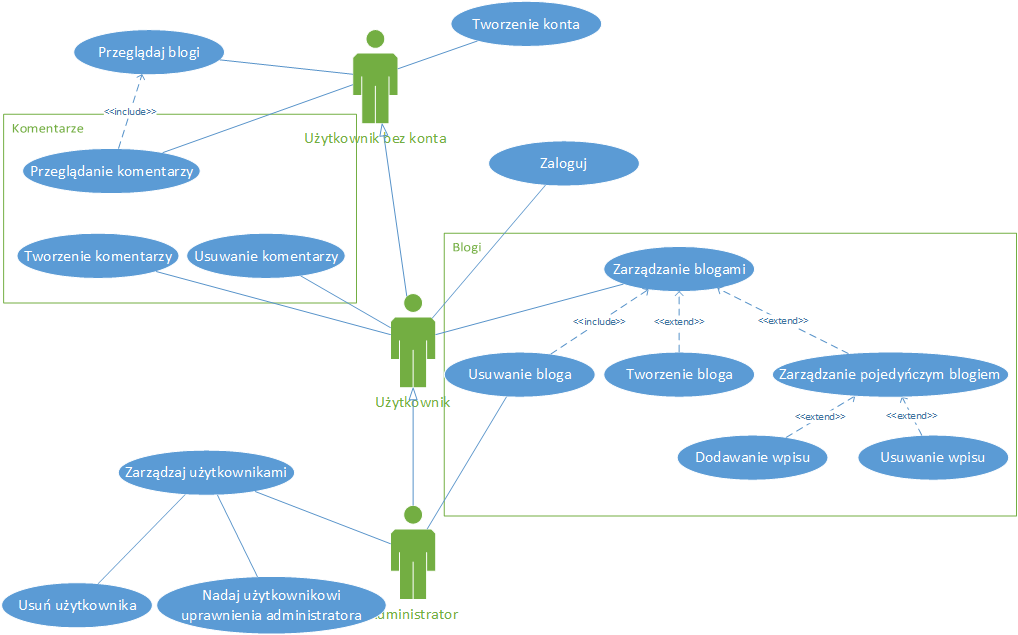
\includegraphics[width=\textwidth]{UseCaseDiagram}
%next-next exam
\section{Diagram klas}
\subsection{Diagram repozytoriów}
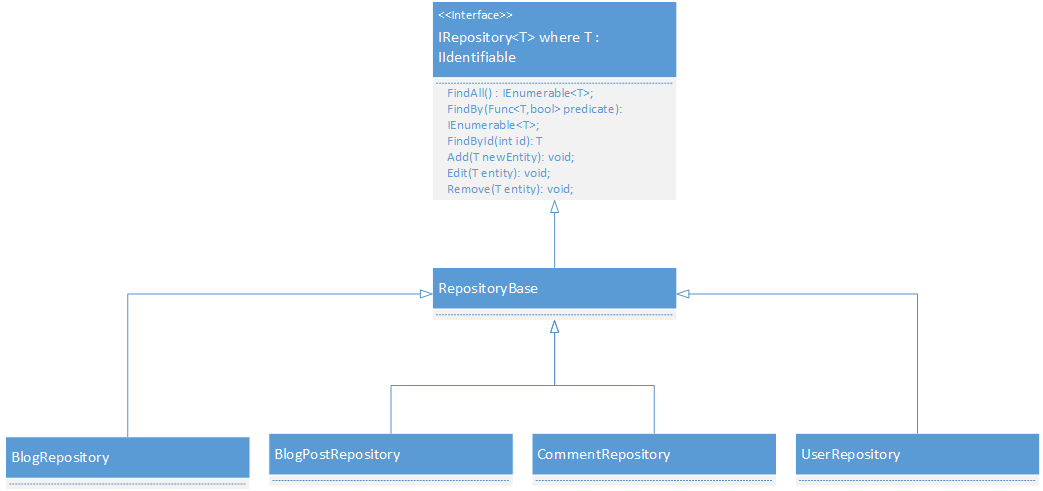
\includegraphics[width=\textwidth]{RepositoryClassDiagram}
\subsection{Diagram modelu}
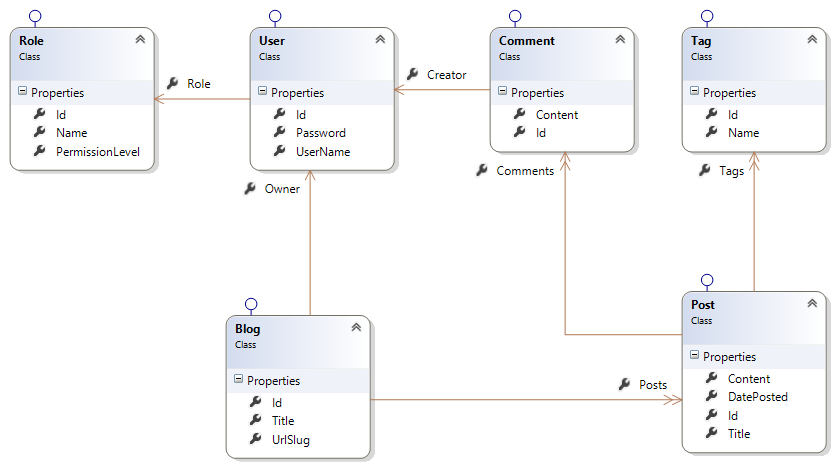
\includegraphics[width=\textwidth]{ModelClassDiagram}
\section{Diagram komponentów}
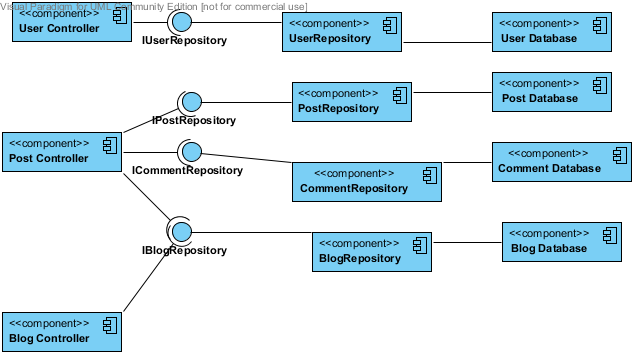
\includegraphics[width=\textwidth]{ComponetDiagram}
\section{Diagram ERD}
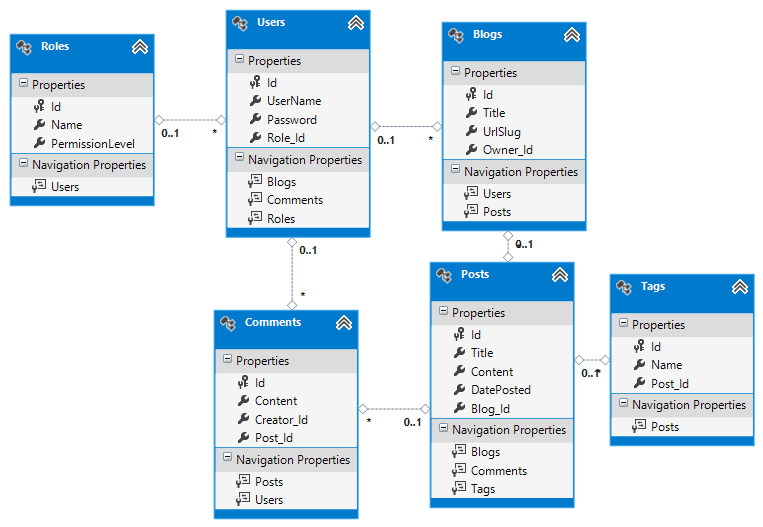
\includegraphics[width=\textwidth]{ERD}
\section{SQL tworzenie bazy danych}
\lstinputlisting[language=SQL]{create_tables.sql}
\end{document}

